
\section{Chapter 1: STEAM}
\subsection{What is Steam?}
Steam is the gas formed when water passes from the liquid to the gaseous state.
At the molecular level, this is when $H_2O$ molecules manage to break free from the bonds 
(i.e. hydrogen bonds) keeping them together\cite{what_is_steam}\relax.


\subsection{Types of Steam:}

\begin{figure}[h!]
    \centering
    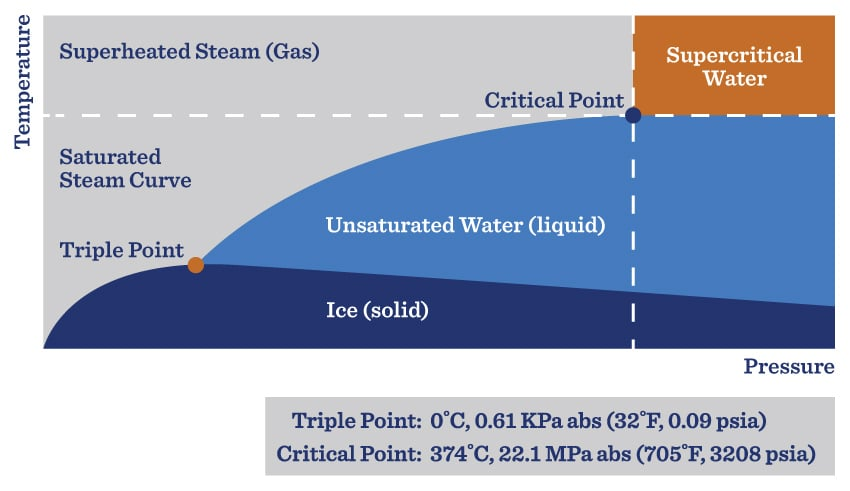
\includegraphics[width=\linewidth]{figs/steam.jpg}
    \caption{Pressure-Temperature Relationship of Water \& Steam}
    \label{fig:webimage}
\end{figure}
\textbf{1. Saturated Steam:} Saturated steam is steam that has reached its boiling point. 
The most typical example is steam at atmospheric pressure, when saturated steam would be at 212°F (100°C). 
It is the steam that is most often employed, particularly in the pharmaceutical industry.\\
\textbf{2.	Superheated Steam:} As the name implies, superheated steam is steam that has been heated over its boiling point at a certain pressure.
Despite being hotter than 100°C, superheated steam would maintain the same atmospheric pressure. \\
\textbf{3.	Dry Steam:} No liquid is present in dry steam, which is entirely in the vapor phase. Since any liquid is immediately heated, superheated steam is dry.
In general, saturated steam is dry, therefore getting rid of the water and using the steam requires a good steam trap. \\
\textbf{4.	Wet steam:} Unsaturated steam, commonly referred to as wet steam, is made up of both water and vapor.
Since wet steam has already lost its vaporization heat, it cannot transport heat effectively. 

\subsection{Application of Steam}
There are many industry verticles wheere steam is used, below are some of the areas where steam is used extensively.
\begin{enumerate}
    \item Textile industry
    \item Food \&\ Beverage industry
    \item Ceremic industry
    \item Sugar industry
    \item Pulp industry
    \item Dairy industry
\end{enumerate}